\documentclass[a4paper, 12pt]{article}

\usepackage[utf8]{inputenc}
\usepackage[T1]{fontenc}
\usepackage[english]{babel}
\usepackage{amsmath, amssymb}
\usepackage{graphicx}
\usepackage{listings}
\usepackage[margin=0.75in, top=0.75in, bottom=0.75in]{geometry}  % Reduce all margins
\usepackage{color}
\usepackage{float}
\usepackage{hyperref}

% Define code listing settings
\lstset{
    basicstyle=\ttfamily\small,
    breaklines=true,
    numbers=left,
    numberstyle=\tiny,
    frame=single,
    language=Python,
}

\title{Neural Learning - 76909 Problem Set 1}
\author{Hadar Tal}
\date{\today}

\begin{document}

\maketitle

\section*{Task 3: The Perceptron Algorithm}

\subsection*{3.1 Binary Perceptron}
I have implemented the function in Python:
\begin{lstlisting}
    perceptron(X, y0) ==> [w, converged, epochs]
\end{lstlisting}
The figure below demonstrates the result of the algorithm in 2D:

\begin{figure}[h]
    \centering
    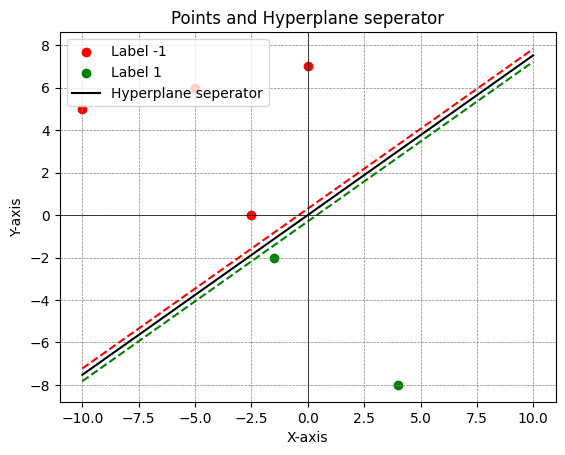
\includegraphics[width=0.6\textwidth]{./assets/nn_ex1_3_1.png}
\end{figure}

\subsection*{3.2 Binary Perceptron Learning Algorithm (for $P < N$)}
The graph below illustrates the relationship between $N$ (points' dimension) and the 
number of epochs required for convergence ($P=10$ for all iterations). 
From the graph, we can infer that the number of epochs decreases as $N$ increases until some $\hat{N}$, 
where for all $n > \hat{N}$, it becomes approximately a constant number. 
As seen in class, for $P < N$, an optimal $w$ is of the form:
\[ w^\star = \sum_{\mu = 1}^{P} (Q^{-1}y_0)_{\mu} x^{\mu} + w_{\bot }\]
where $w_{\bot }$ is an arbitrary vector perpendicular to all examples, 
and ${Q}_{\mu \nu } \equiv  {(x^\mu)}^T x^\nu$. 
As the dimensionality increases, the volume of the space grows exponentially. 
In higher-dimensional spaces, points become more spread out, and it becomes easier to find a hyperplane that separates them.

\begin{figure}[h]
    \centering
    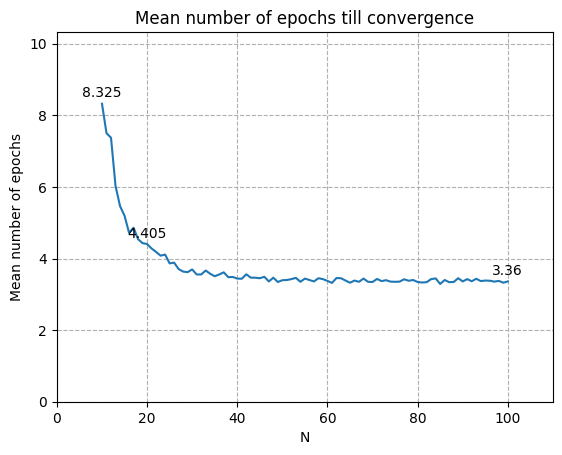
\includegraphics[width=0.6\textwidth]{./assets/nn_ex1_3_2_1.png}
\end{figure}

\subsection*{3.3 Estimation of the Perceptron's Capacity as a Function of $\alpha = \frac{P}{N}$}
The plots below show the probability of convergence as a function of $0 < \alpha < 3$ for $N = 5, 20, 100$.

\begin{figure}[h]
    \centering
    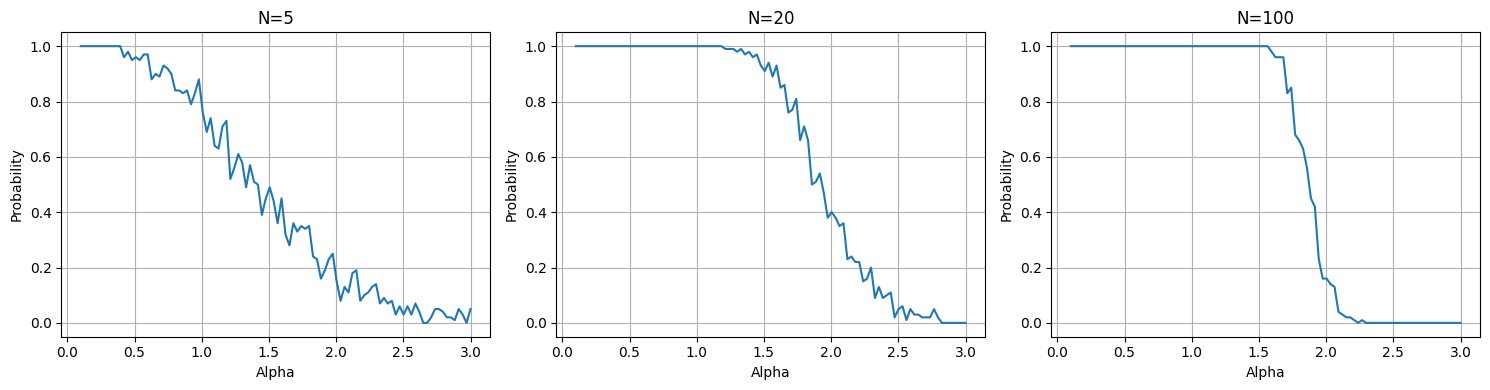
\includegraphics[width=1\textwidth]{./assets/nn_ex1_3_3_1.png}
\end{figure}

We observe a threshold phenomenon for this probability. Cover's function counting theorem states that if $\{x^1, \dots, x^P\}$ is a set of vectors in 
$\mathbb{R} ^N$ in general position, the number of dichotomies that can be performed 
using a plane that goes through the origin is given by:
\[ C(P,N) = 2 \sum_{k=0}^{N-1} \binom{P-1}{k} \]
When estimating the probability of convergence, we approximate dividing this term
by all the possibilities to spread the $P$ points in the $N$ dimensional space. 
For $0 < \alpha < 1$, it is the same case where $P < N$, and all dichotomies can 
be realized. For $\alpha = 2$, we have seen that exactly half of all the possible dichotomies can be realized.
And for $P \gg N$, the total number of realizable dichotomies is $\sim P^N$, but the total 
number of dichotomies is $2^P$. We can see that $\alpha \rightarrow  3 \implies Prob \rightarrow 0$.

\vspace{24pt} 

The $t_{\text{max}}$ parameter defines the maximal number of epochs before the perceptron
returns that it didn't converge. Increasing this parameter will possibly lead to 
an increase in the probability of convergence, but up to a constant. The probability 
is determined by the argument we have mentioned above - the actual capacity of 
the perceptron. 
The demonstration below shows that some values larger than $10^3$ don't have a major impact
on the results.

\begin{figure}[h]
    \centering
    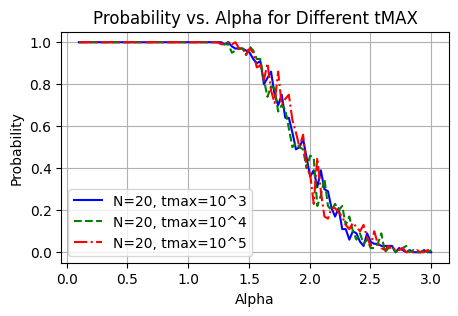
\includegraphics[width=0.6\textwidth]{./assets/nn_ex1_3_3_2.png}
\end{figure}

\end{document}
